\texttt{array}は配列です。この定義は以下のようになります:

\begin{lstlisting}[numbers=none]
var arr [n]type
\end{lstlisting}

\texttt{[n]type}の中で、\texttt{n}は配列の長さを表しています。\texttt{type}は保存する要素の型を示しています。配列に対する操作は他の言語とよく似ていて、どれも\texttt{[]}を通して値の取得および代入を行います。

\begin{lstlisting}[numbers=none]
var arr [10]int  // int型の配列を宣言します。
arr[0] = 42      // 配列のインデックスは0からはじまります。
arr[1] = 13      // 代入操作
fmt.Printf("The first element is %d\n", arr[0])
                 // データを取得して、42を返します。
fmt.Printf("The last element is %d\n", arr[9])
                 // 値が代入されていない最後の要素を返します。
                 // デフォルトでは0が返ります。
\end{lstlisting}

長さも配列の一部ですので、\texttt{[3]int}と\texttt{[4]int}は異なる型になります。配列も長さを変えることはできません。配列間の代入は値渡しです。つまり、一つの配列が関数の引数となった場合、渡されるのは実はこの配列のコピーであり、ポインタではありません。もしポインタを使いたい場合は、この後にご紹介する\texttt{slice}型をご利用ください。

配列はもうひとつの\texttt{:=}で宣言することができます。

\begin{lstlisting}[numbers=none]
a := [3]int{1, 2, 3} // 長さが3のintの配列を宣言します。

b := [10]int{1, 2, 3} // 長さが10のint配列を宣言します。
                      // この中で3つの要素の初期値は1、2、3で、
                      // そのほかのデフォルトは0です。

c := [...]int{4, 5, 6} // 長さを`...`で省略することも
                      // できます。Goは自動で要素数から長さを
                      // 計算します。
\end{lstlisting}

もしあなたが「配列に配列を込めたい場合は実現できますか?」と問うならば、当然ですとも、とお応えしましょう。Goはネストした配列をサポートしています。例えば下のコードでは二次元配列を宣言しています:


\begin{lstlisting}[numbers=none]
  // 二次元配列を一つ宣言します。この配列は
  // 2つの配列を要素としており、各配列には4つ
  // のint型の要素が含まれます。
doubleArray := [2][4]int{[4]int{1, 2, 3, 4},
                           [4]int{5, 6, 7, 8}}

    // 上の宣言は簡略化できます。直接内部の型を省略しています。
easyArray := [2][4]int{{1, 2, 3, 4}, {5, 6, 7, 8}}
\end{lstlisting}

配列の状態は以下のとおりです:

\begin{figure}[H]
  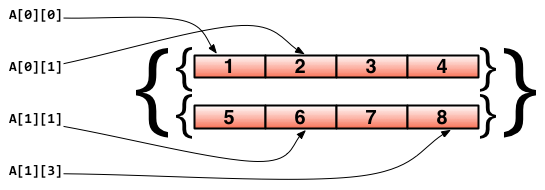
\includegraphics[width=14cm]{2.2.array.png}
   \label{図2.2}
   \caption{多次元配列のマッピング関係}
\end{figure}

